% Created 2021-09-11 Sat 16:43
% Intended LaTeX compiler: xelatex
\documentclass[letterpaper]{article}
\usepackage{graphicx}
\usepackage{grffile}
\usepackage{longtable}
\usepackage{wrapfig}
\usepackage{rotating}
\usepackage[normalem]{ulem}
\usepackage{amsmath}
\usepackage{textcomp}
\usepackage{amssymb}
\usepackage{capt-of}
\usepackage{hyperref}
\usepackage[margin=1in]{geometry}
\usepackage{fontspec}
\usepackage{indentfirst}
\setmainfont[ItalicFont = LiberationSans-Italic, BoldFont = LiberationSans-Bold, BoldItalicFont = LiberationSans-BoldItalic]{LiberationSans}
\newfontfamily\NHLight[ItalicFont = LiberationSansNarrow-Italic, BoldFont       = LiberationSansNarrow-Bold, BoldItalicFont = LiberationSansNarrow-BoldItalic]{LiberationSansNarrow}
\newcommand\textrmlf[1]{{\NHLight#1}}
\newcommand\textitlf[1]{{\NHLight\itshape#1}}
\let\textbflf\textrm
\newcommand\textulf[1]{{\NHLight\bfseries#1}}
\newcommand\textuitlf[1]{{\NHLight\bfseries\itshape#1}}
\usepackage{fancyhdr}
\pagestyle{fancy}
\usepackage{titlesec}
\usepackage{titling}
\makeatletter
\lhead{\textbf{\@title}}
\makeatother
\rhead{\textrmlf{Compiled} \today}
\lfoot{\theauthor\ \textbullet \ \textbf{2021-2022}}
\cfoot{}
\rfoot{\textrmlf{Page} \thepage}
\titleformat{\section} {\Large} {\textrmlf{\thesection} {|}} {0.3em} {\textbf}
\titleformat{\subsection} {\large} {\textrmlf{\thesubsection} {|}} {0.2em} {\textbf}
\titleformat{\subsubsection} {\large} {\textrmlf{\thesubsubsection} {|}} {0.1em} {\textbf}
\setlength{\parskip}{0.45em}
\renewcommand\maketitle{}
\author{Exr0n}
\date{\today}
\title{ret More Systems and Proofs}
\hypersetup{
 pdfauthor={Exr0n},
 pdftitle={ret More Systems and Proofs},
 pdfkeywords={},
 pdfsubject={},
 pdfcreator={Emacs 27.2 (Org mode 9.4.4)}, 
 pdflang={English}}
\begin{document}

\maketitle


\section{Solve Equations}
\label{sec:orgb1eef4b}
Operation timed out. Arithmetic errors. \#todo

\begin{center}
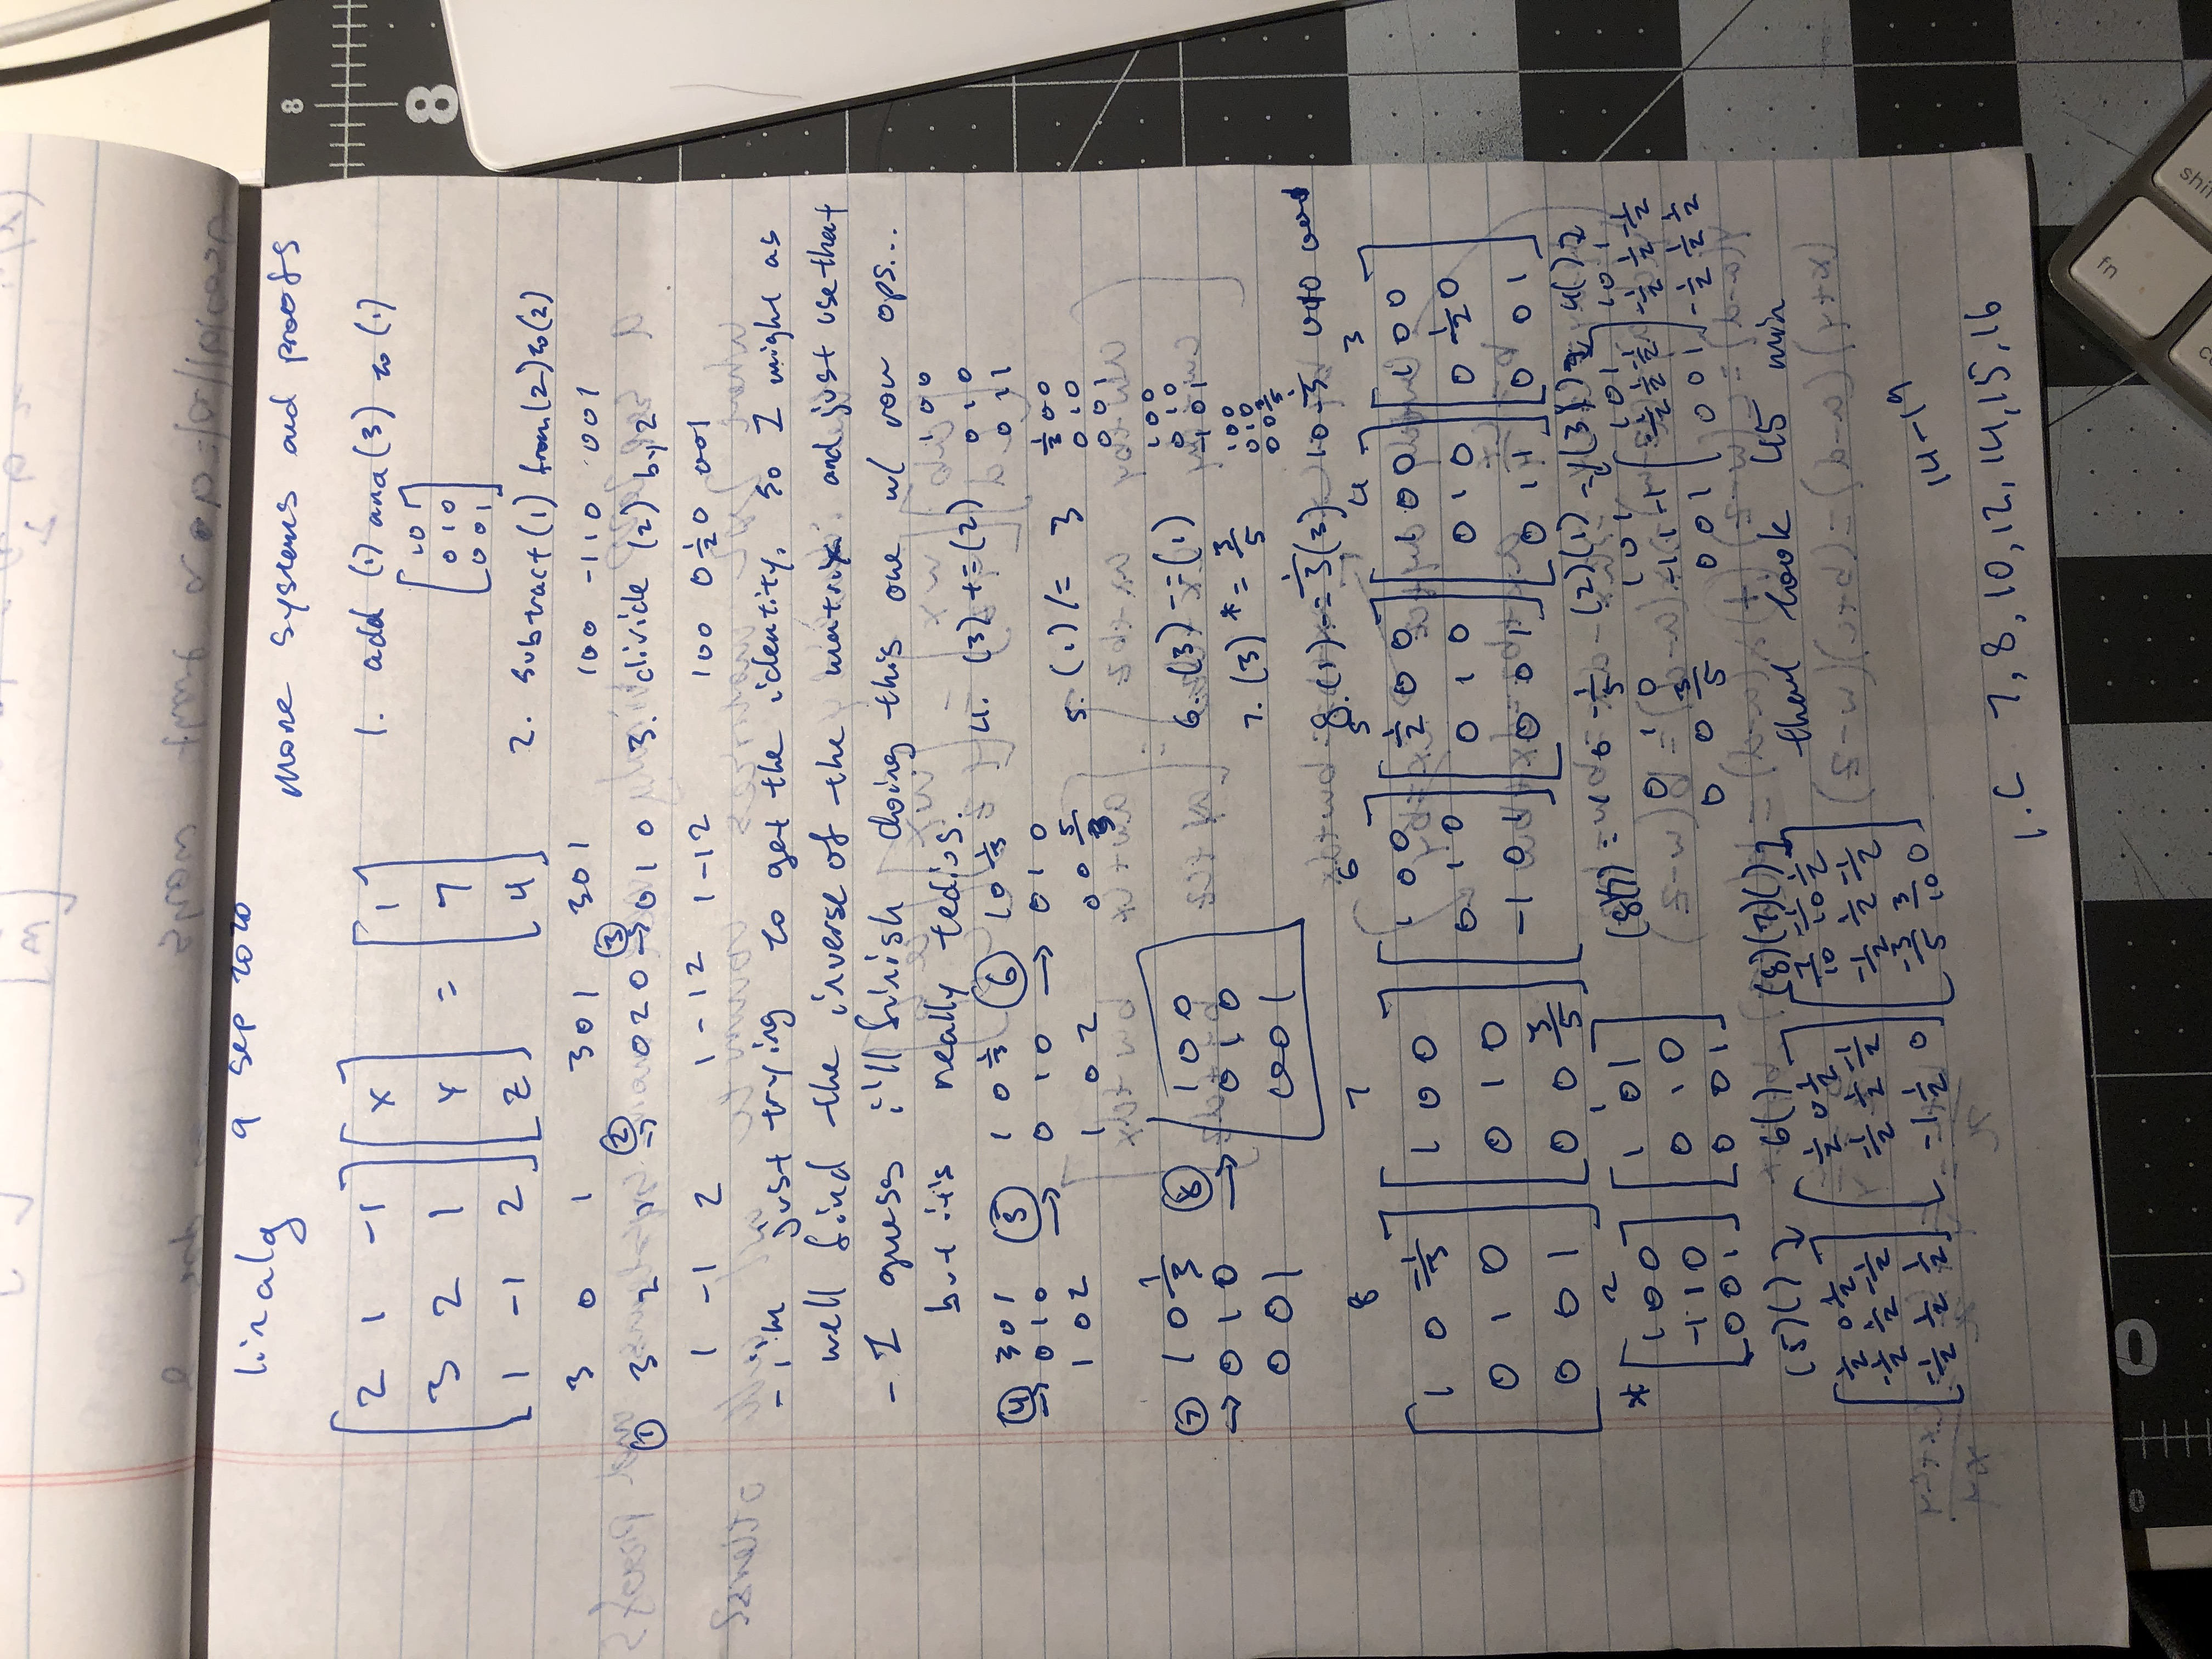
\includegraphics[width=.9\linewidth]{IMG_1379.jpg}
\end{center}

\section{Read 1.B and 1.C}
\label{sec:orga0f6ee4}
\subsection{General Notes}
\label{sec:org71654fa}
\begin{itemize}
\item The distributive property is extremely useful \#\#\# 1.35 Example

\item \begin{enumerate}
\item If \(b = 0\) then we can divide all \(x_3\) by \(5\) and combine
the last two terms to get \(F^3\), which is a vector space, without
loss of generality. If not, then when you try to multiply by a
scalar then you will find that the above reasoning breaks (i
think).
\end{enumerate}

\item \begin{enumerate}
\item \(f(x) = 0\) is continuous, so the additive identity exists. All
sums of continuous functions result in continuous functions, so it
is closed under addition. And all scalar multiples also work out.
\end{enumerate}

\item \begin{enumerate}
\item slightly awkward: i don't actually know what a differentiable real
valued function is. \#todo-exr0n
\end{enumerate}

\item \begin{enumerate}
\item (see previous)
\end{enumerate}

\item \begin{enumerate}
\item what does it mean for a sequence of complex numbers to have a limit
\(0\)? but I think you can use the same argument that the missing
elements are just "collapsed" into one invisible one. \#\#\# 1.40
Definition direct sum
\end{enumerate}

\item Something about uniqueness?

\item If there is only one way to write zero then it works (1.44 Condition
for a direct sum)
\end{itemize}

\subsection{Exercise to present}
\label{sec:org5a8179d}
I would be interested in 7, 8, 10, 12, 14-19

\section{2x2 Matrices that are Commutative}
\label{sec:org0a12557}
(under multiplication, with all other 2x2 matrices)

Starting with
\(\begin{bmatrix}a&b\\c&d\end{bmatrix}\begin{bmatrix}w&x\\y&z\end{bmatrix}=\begin{bmatrix}w&x\\y&z\end{bmatrix}\begin{bmatrix}a&b\\c&d\end{bmatrix}\),
I got \((x+y)(a-d) = (b+c)(w-z)\) and \(by=cx\), but wasn't sure how to
further develop it.

\begin{center}
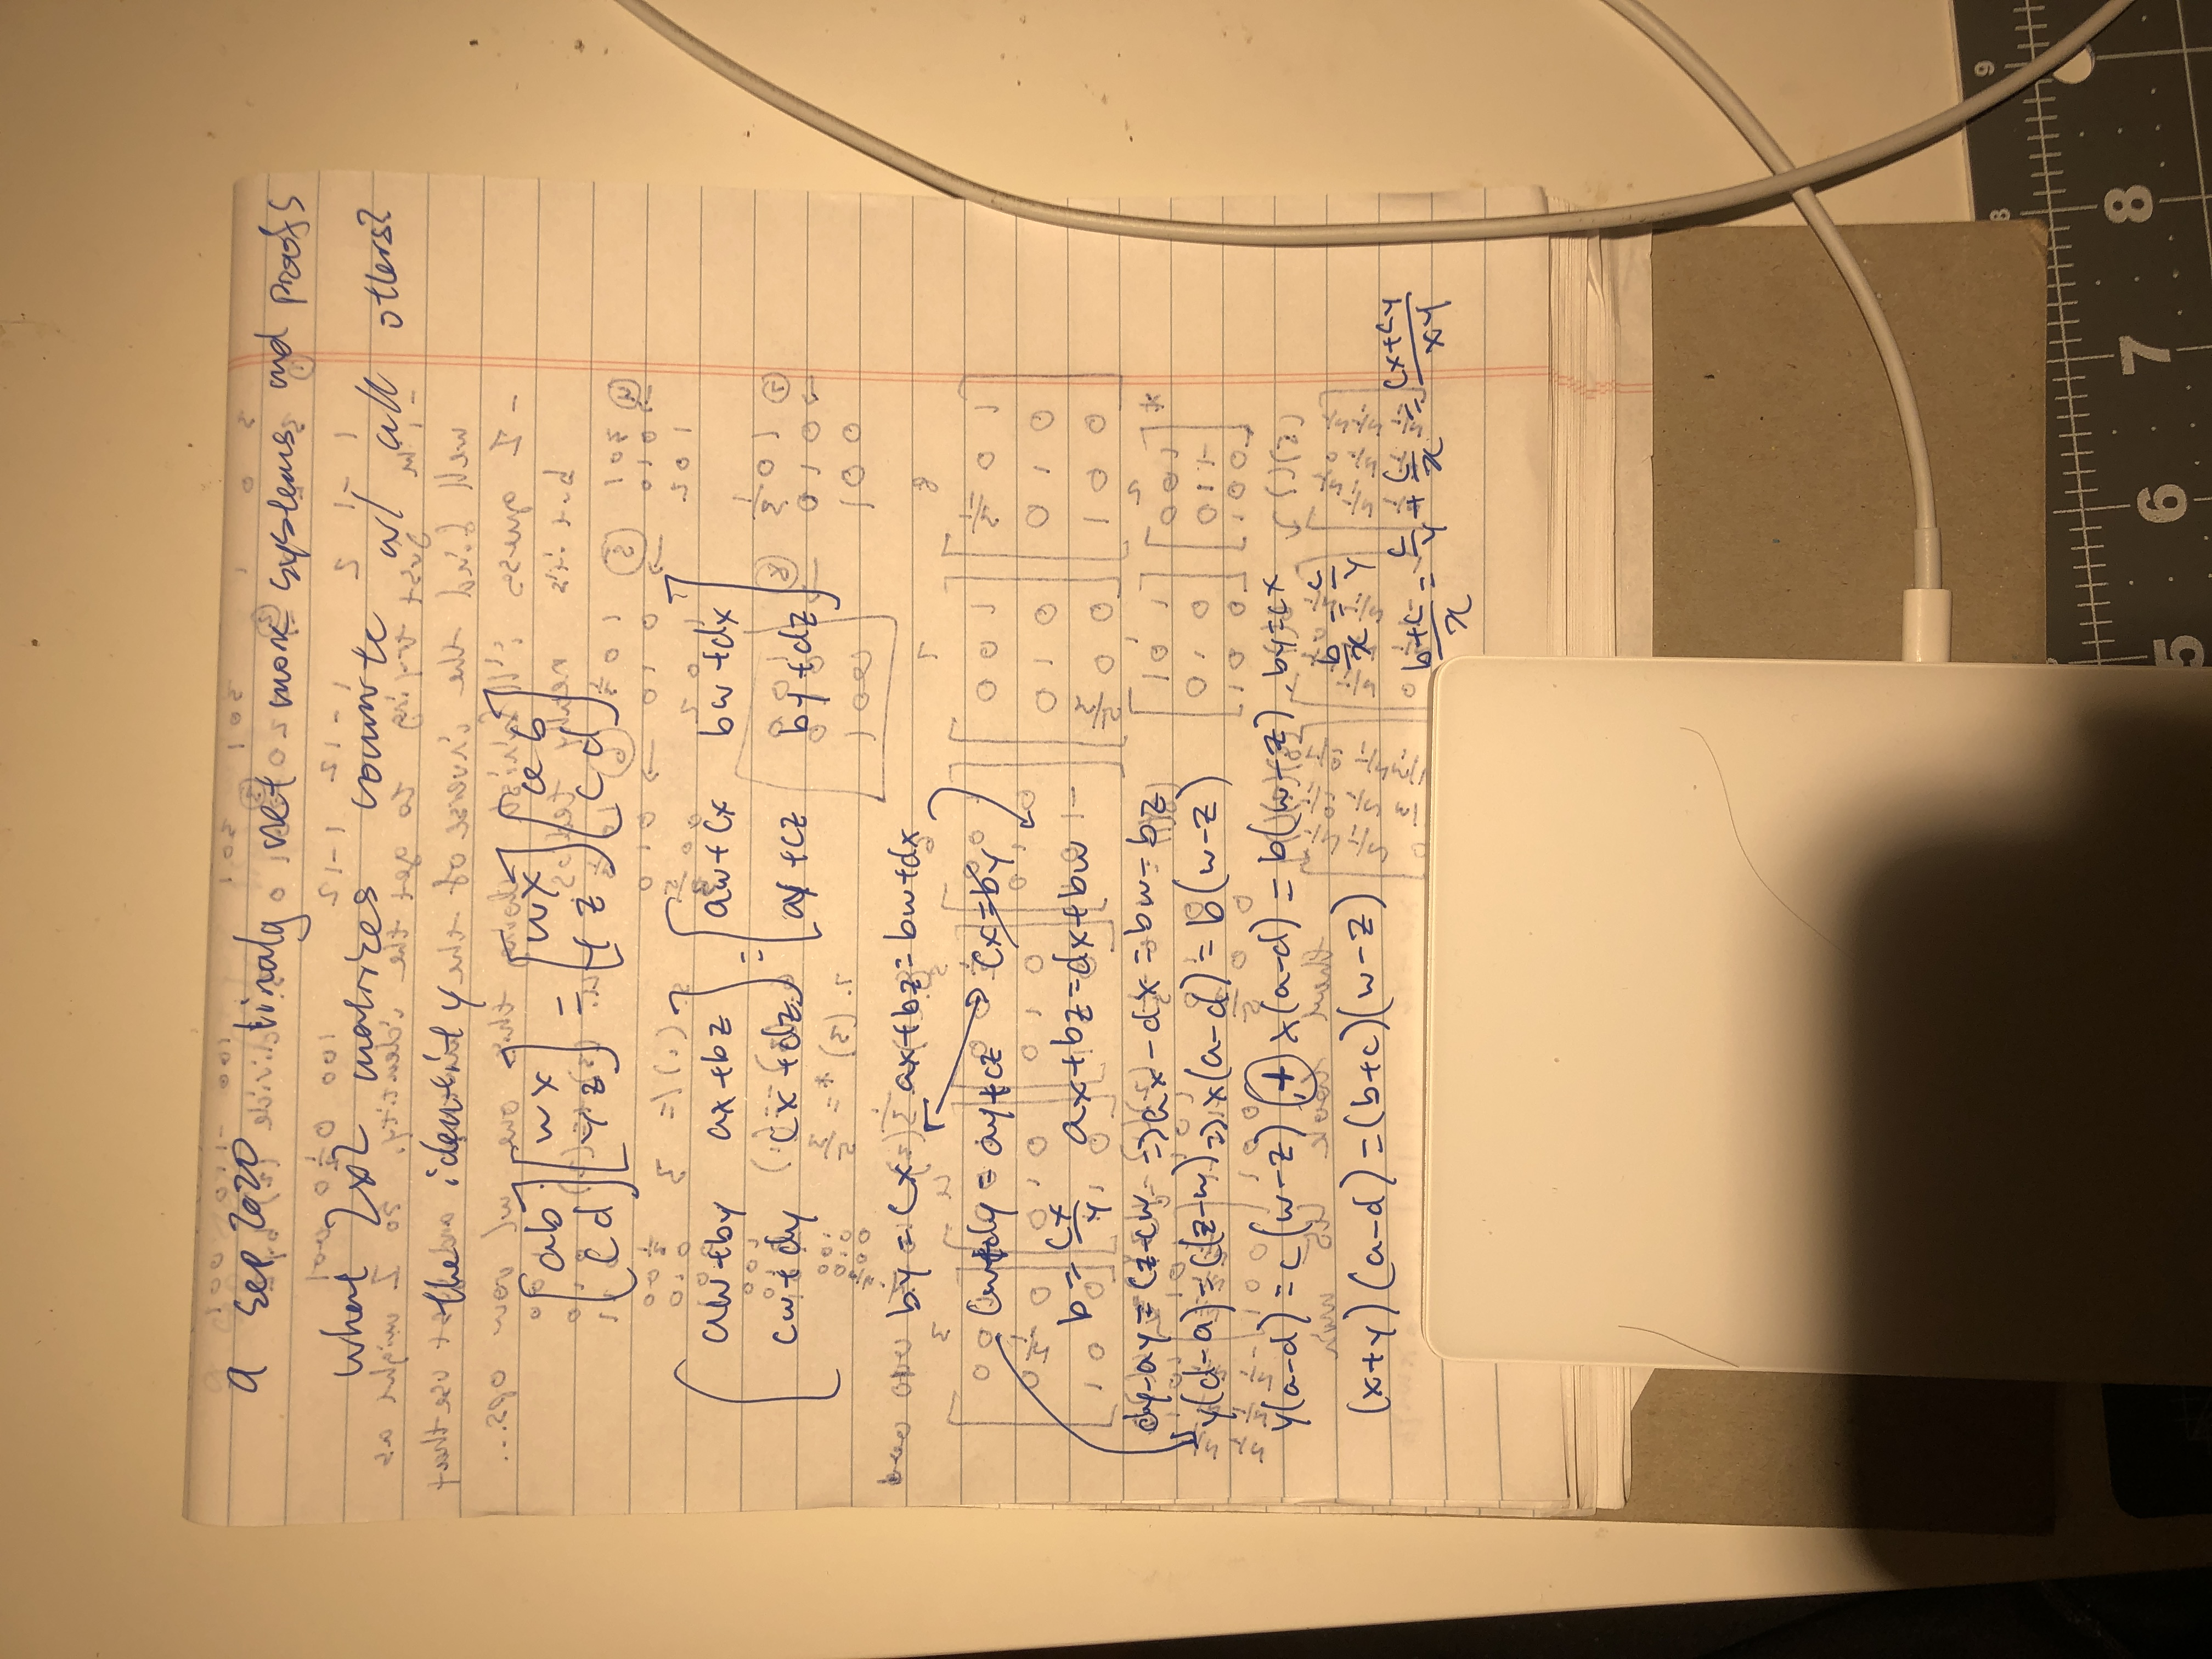
\includegraphics[width=.9\linewidth]{IMG_1380.jpg}
\end{center}

\section{Epilogue}
\label{sec:org819d840}
Linear algebra homework always takes so long. Even though I skip like
half of the problems. This is kind of an issue.

\noindent\rule{\textwidth}{0.5pt}
\end{document}
